\section{原理}

\subsection{点接触におけるヘルツの弾性接触理論}
縦弾性係数$E_1$,$E_2$,ポアソン比$\nu_1$,$\nu_2$,半径$R_1$,$R_2$の二つの球が荷重$W$で接触する場合の圧力分布は点対象であり,接触部は円形となる(図\ref{fig:fig_ヘルツ接触}).この場合の圧力分布,ヘルツ最大接触圧力,平均接触圧力,接触円半径,接触中心の変形量の関係式をそれぞれ式(\ref{eq:圧力分布})から式(\ref{eq:接触中心の変形量})にかけて示す.
\begin{equation}
    \label{eq:圧力分布}
    p = P_{max}\sqrt{1 - (\frac{r}{a})^2}
\end{equation}
\begin{equation}
    \label{eq:最大接触圧力}
    P_{max} = \frac{3W}{2\pi a^2}
\end{equation}
\begin{equation}
    \label{eq:平均接触圧力}
    P_{m} = \frac{W}{\pi a^2} = \frac{2}{3}P_{max}
\end{equation}
\begin{equation}
    \label{eq:接触円半径}
    a = \sqrt[3]{\frac{3W}{4} \frac{R}{E}}
\end{equation}
\begin{equation}
    \label{eq:接触中心の変形量}
    \delta = \frac{a^2}{R}
\end{equation}
ここで,$p$,$P_{max}$,$P_{m}$の単位は[Pa]であり,$a$,$\delta$の単位は[m]である.また,$R$及び$E$は等価半径及び等価縦弾性係数とよばれ,次のように定義される.
\begin{equation}
    \label{eq:等価半径}
    \frac{1}{R} = \frac{1}{R_1} + \frac{1}{R_2}
\end{equation}
\begin{equation}
    \label{eq:等価縦弾性係数}
    \frac{1}{E} = \frac{1 - \nu_1^2}{E_1} + \frac{1 - \nu_2^2}{E_2}
\end{equation}
\begin{figure}[htbp]
    \centering %中央揃え
    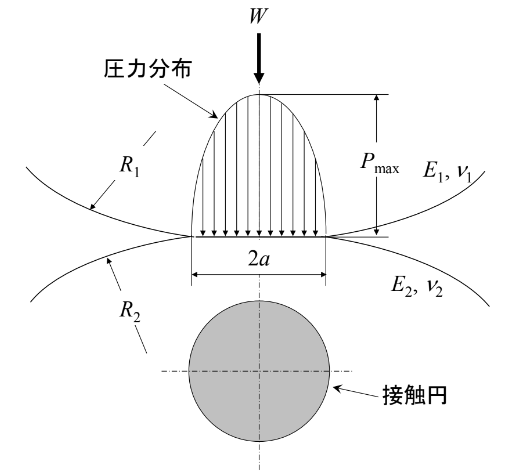
\includegraphics[width=100truemm,clip]{fig/fig_ヘルツ接触.png}
    \caption{Hertzian contact in a point contact.}
    \label{fig:fig_ヘルツ接触}
\end{figure}

\subsection{ビッカース硬さ}
ビッカース硬さとは,対面角 136$^\circ$の正四角錘ダイヤモンド圧子を用いて,試験面にピラミッド形のくぼみ(図\ref{fig:ビッカース硬さ})をつけたときの荷重を,永久くぼみの対角線の長さから求めた表面積で除した値をいい,次の式で算出される.
\begin{figure}[htbp]
    \centering %中央揃え
    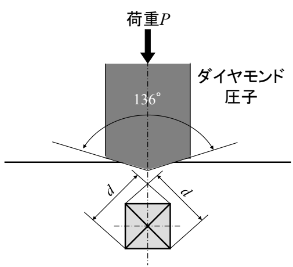
\includegraphics[width=100truemm,clip]{fig/fig_ビッカース硬さ.png}
    \caption{Vickers indenter and indentation.}
    \label{fig:ビッカース硬さ}
\end{figure}
\begin{equation}
    \label{eq:ビッカース硬さ}
    \mathrm{H_v} = \frac{P}{S} = \frac{2Psin \frac{\alpha}{2}}{d^2} = 1.854\frac{P}{d^2}
\end{equation}
ここで,$\mathrm{H_v}$はビッカース硬さ[$\mathrm{kgf/mm^2}$],$P$は荷重[$\mathrm{kgf}$],$S$はくぼみの表面積[$\mathrm{mm^2}$],$d$はくぼみ対角線の長さの平均値[mm],$\alpha$は対面角[$^\circ$]である. この硬さの単位は$\mathrm{kgf/mm^2}$であるが,換算してGPaが用いられる場合も多い.

\subsection{球と平面の静的接触における基本的な3形態}
理想的に滑らかな平面と球との静的接触の形態は,弾性接触,弾塑性接触,塑性接触の3種類に分類される.分類をまとめたものを図に示す.

\begin{figure}[htbp]
    \centering %中央揃え
    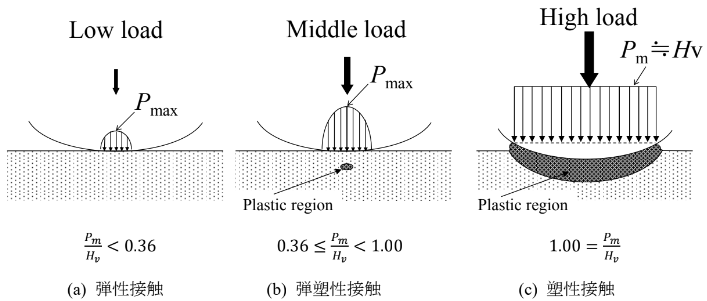
\includegraphics[width=100truemm,clip]{fig/fig_接触形態の分類.png}
    \caption{Classification of contact morphology in static contact.}
    \label{fig:接触形態}
\end{figure}

\subsection{すべり摩擦の機構}

\subsubsection{凝着項}
摩擦面同士が相対すべり運動するためには,真実接触部での凝着部分をせん断することが必要であり,このせん断力$F_a$が摩擦力となる.ここで凝着とは,二つの固体表面が第三の物質を介して,互いに接合する現象のことであり,その結合形態は,共有·金属·イオン結合からなる一次結合と,分子間力を主体とした二次結合に分類される.
\begin{equation}
    \label{eq:せん断力}
    F_A = A_\tau \tau
\end{equation}
ここで$A_\tau$は真実接触面積,$\tau$は凝着部をせん断するために必要な界面のせん断応力[Pa]である.

\subsubsection{掘り起こし項}
硬い金属の突起が軟らかい金属の中に押し込まれた状態で互いにすべるためには,前面にある部分を排除,すなわちすき起こさなければならない.これに必要な力 $F_p$が摩擦力となり,次のように表すことができる.
\begin{equation}
    \label{eq:掘り起こし}
    F_p = A_h p_0
\end{equation}
ここで,$A_h$は進行方向前面の投影面積[$\mathrm{m^2}$],$p_0$は塑性流動圧力[Pa]である.

摩擦力は$F = F_a + F_h$と表されるが,一般に機械要素として表される摩擦面の表面粗さは小さいため,掘り起こし項は凝着項に比較して小さく無視できる.したがって,摩擦係数$\mu$は次のように表される.
\begin{equation}
    \label{eq:摩擦係数}
    \mu = \frac{F}{W} \approx \frac{F_a}{W} = \frac{A_\tau \tau}{W}
\end{equation}